% figures/figA_resolution.tex -- float wrapper for the APPENDIX resolution figure.
%
% NOT YET INPUT ANYWHERE.  This wrapper is written and ready; the section editor
% adds it to the appendix (Appendix B.6, the numerics discussion) with
%     % figures/figA_resolution.tex -- float wrapper for the APPENDIX resolution figure.
%
% NOT YET INPUT ANYWHERE.  This wrapper is written and ready; the section editor
% adds it to the appendix (Appendix B.6, the numerics discussion) with
%     % figures/figA_resolution.tex -- float wrapper for the APPENDIX resolution figure.
%
% NOT YET INPUT ANYWHERE.  This wrapper is written and ready; the section editor
% adds it to the appendix (Appendix B.6, the numerics discussion) with
%     % figures/figA_resolution.tex -- float wrapper for the APPENDIX resolution figure.
%
% NOT YET INPUT ANYWHERE.  This wrapper is written and ready; the section editor
% adds it to the appendix (Appendix B.6, the numerics discussion) with
%     \input{figures/figA_resolution}
% It must NOT go in the main text: the nine-page main text has no vertical slack
% and this figure is a diagnostic, not a result.
%
% Image produced by figures/figA_resolution.py, which also writes
% figures/out/figA_resolution_data.json recording every number drawn.
%
% PROVENANCE.  The per-checkpoint values are the authoritative re-scoring of the
% records under runs/eval_res/{a1_fm_only,a3_energy_only}[_s<N>]__ode{4,12,48};
% they are transcribed, not recomputed, per the standing instruction.  The
% generator recomputes every AGGREGATE (arm means, gaps, Welch t) from those
% per-checkpoint values and refuses to draw unless each reproduces the
% authoritative aggregate; it also checks the two directional counts the figure
% states before stating them.  The Welch t values stay inside that gate and
% inside figA_resolution_data.json: NO t value and NO significance label is
% rendered in the image or in the caption.  Panel (b) is descriptive -- the
% difference of arm means with the propagated SEM over seeds.
%
% Drawn at final size (5.5 x 2.42 in) with an explicit, non-tight bounding box;
% include with width=\linewidth, never \resizebox.
\begin{figure}[t]
\begin{center}
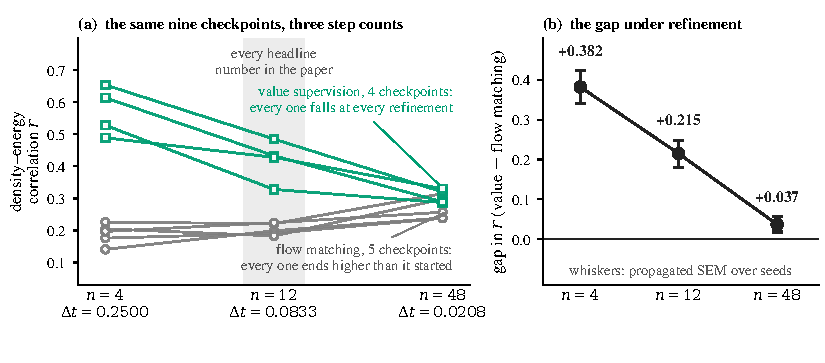
\includegraphics[width=\linewidth]{figures/out/figA_resolution.pdf}
\end{center}
\caption{\textbf{The paired resolution sweep.} The same nine checkpoints ---
five flow-matching controls (seeds $1$--$5$) and four value runs (seeds
$1$, $2$, $3$, $5$) --- re-scored at $n = 4$, $n = 12$ and $n = 48$ ODE steps on
identical parents, identical displacements and a pinned evaluation seed.
\textbf{(a)} Per checkpoint: all four value checkpoints fall at every
refinement, and all five flow-matching checkpoints end higher at $n = 48$ than
at $n = 4$, three of them monotonically. \textbf{(b)} The arm gap decays
$+0.382 \rightarrow +0.215 \rightarrow +0.037$. Each point is the difference of
the two arm means over independently trained seeds, five control and four
value, and each whisker is the propagated standard error over those seeds, a
descriptive SEM rather than a confidence interval. Every number reported
elsewhere in the paper is computed at $n = 12$. The value loss was itself
computed at $n = 4$, so one reading of the decay is that the ordering the term
teaches is expressed most strongly in the object the coarse estimator reports;
that is offered as a reading and not as a demonstrated mechanism. What the
analysis establishes is that the estimator is sensitive to solver resolution.
It does not distinguish model-dependent numerical error from an effect learned
under the four-step training estimator.}
\label{fig:resolution}
\end{figure}

% It must NOT go in the main text: the nine-page main text has no vertical slack
% and this figure is a diagnostic, not a result.
%
% Image produced by figures/figA_resolution.py, which also writes
% figures/out/figA_resolution_data.json recording every number drawn.
%
% PROVENANCE.  The per-checkpoint values are the authoritative re-scoring of the
% records under runs/eval_res/{a1_fm_only,a3_energy_only}[_s<N>]__ode{4,12,48};
% they are transcribed, not recomputed, per the standing instruction.  The
% generator recomputes every AGGREGATE (arm means, gaps, Welch t) from those
% per-checkpoint values and refuses to draw unless each reproduces the
% authoritative aggregate; it also checks the two directional counts the figure
% states before stating them.  The Welch t values stay inside that gate and
% inside figA_resolution_data.json: NO t value and NO significance label is
% rendered in the image or in the caption.  Panel (b) is descriptive -- the
% difference of arm means with the propagated SEM over seeds.
%
% Drawn at final size (5.5 x 2.42 in) with an explicit, non-tight bounding box;
% include with width=\linewidth, never \resizebox.
\begin{figure}[t]
\begin{center}
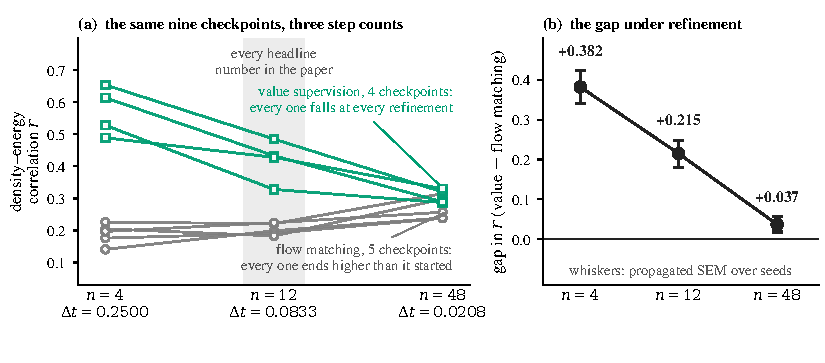
\includegraphics[width=\linewidth]{figures/out/figA_resolution.pdf}
\end{center}
\caption{\textbf{The paired resolution sweep.} The same nine checkpoints ---
five flow-matching controls (seeds $1$--$5$) and four value runs (seeds
$1$, $2$, $3$, $5$) --- re-scored at $n = 4$, $n = 12$ and $n = 48$ ODE steps on
identical parents, identical displacements and a pinned evaluation seed.
\textbf{(a)} Per checkpoint: all four value checkpoints fall at every
refinement, and all five flow-matching checkpoints end higher at $n = 48$ than
at $n = 4$, three of them monotonically. \textbf{(b)} The arm gap decays
$+0.382 \rightarrow +0.215 \rightarrow +0.037$. Each point is the difference of
the two arm means over independently trained seeds, five control and four
value, and each whisker is the propagated standard error over those seeds, a
descriptive SEM rather than a confidence interval. Every number reported
elsewhere in the paper is computed at $n = 12$. The value loss was itself
computed at $n = 4$, so one reading of the decay is that the ordering the term
teaches is expressed most strongly in the object the coarse estimator reports;
that is offered as a reading and not as a demonstrated mechanism. What the
analysis establishes is that the estimator is sensitive to solver resolution.
It does not distinguish model-dependent numerical error from an effect learned
under the four-step training estimator.}
\label{fig:resolution}
\end{figure}

% It must NOT go in the main text: the nine-page main text has no vertical slack
% and this figure is a diagnostic, not a result.
%
% Image produced by figures/figA_resolution.py, which also writes
% figures/out/figA_resolution_data.json recording every number drawn.
%
% PROVENANCE.  The per-checkpoint values are the authoritative re-scoring of the
% records under runs/eval_res/{a1_fm_only,a3_energy_only}[_s<N>]__ode{4,12,48};
% they are transcribed, not recomputed, per the standing instruction.  The
% generator recomputes every AGGREGATE (arm means, gaps, Welch t) from those
% per-checkpoint values and refuses to draw unless each reproduces the
% authoritative aggregate; it also checks the two directional counts the figure
% states before stating them.  The Welch t values stay inside that gate and
% inside figA_resolution_data.json: NO t value and NO significance label is
% rendered in the image or in the caption.  Panel (b) is descriptive -- the
% difference of arm means with the propagated SEM over seeds.
%
% Drawn at final size (5.5 x 2.42 in) with an explicit, non-tight bounding box;
% include with width=\linewidth, never \resizebox.
\begin{figure}[t]
\begin{center}
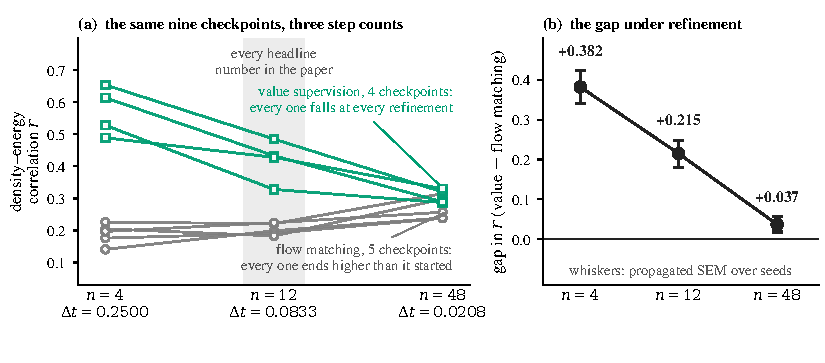
\includegraphics[width=\linewidth]{figures/out/figA_resolution.pdf}
\end{center}
\caption{\textbf{The paired resolution sweep.} The same nine checkpoints ---
five flow-matching controls (seeds $1$--$5$) and four value runs (seeds
$1$, $2$, $3$, $5$) --- re-scored at $n = 4$, $n = 12$ and $n = 48$ ODE steps on
identical parents, identical displacements and a pinned evaluation seed.
\textbf{(a)} Per checkpoint: all four value checkpoints fall at every
refinement, and all five flow-matching checkpoints end higher at $n = 48$ than
at $n = 4$, three of them monotonically. \textbf{(b)} The arm gap decays
$+0.382 \rightarrow +0.215 \rightarrow +0.037$. Each point is the difference of
the two arm means over independently trained seeds, five control and four
value, and each whisker is the propagated standard error over those seeds, a
descriptive SEM rather than a confidence interval. Every number reported
elsewhere in the paper is computed at $n = 12$. The value loss was itself
computed at $n = 4$, so one reading of the decay is that the ordering the term
teaches is expressed most strongly in the object the coarse estimator reports;
that is offered as a reading and not as a demonstrated mechanism. What the
analysis establishes is that the estimator is sensitive to solver resolution.
It does not distinguish model-dependent numerical error from an effect learned
under the four-step training estimator.}
\label{fig:resolution}
\end{figure}

% It must NOT go in the main text: the nine-page main text has no vertical slack
% and this figure is a diagnostic, not a result.
%
% Image produced by figures/figA_resolution.py, which also writes
% figures/out/figA_resolution_data.json recording every number drawn.
%
% PROVENANCE.  The per-checkpoint values are the authoritative re-scoring of the
% records under runs/eval_res/{a1_fm_only,a3_energy_only}[_s<N>]__ode{4,12,48};
% they are transcribed, not recomputed, per the standing instruction.  The
% generator recomputes every AGGREGATE (arm means, gaps, Welch t) from those
% per-checkpoint values and refuses to draw unless each reproduces the
% authoritative aggregate; it also checks the two directional counts the figure
% states before stating them.  The Welch t values stay inside that gate and
% inside figA_resolution_data.json: NO t value and NO significance label is
% rendered in the image or in the caption.  Panel (b) is descriptive -- the
% difference of arm means with the propagated SEM over seeds.
%
% Drawn at final size (5.5 x 2.42 in) with an explicit, non-tight bounding box;
% include with width=\linewidth, never \resizebox.
\begin{figure}[t]
\begin{center}
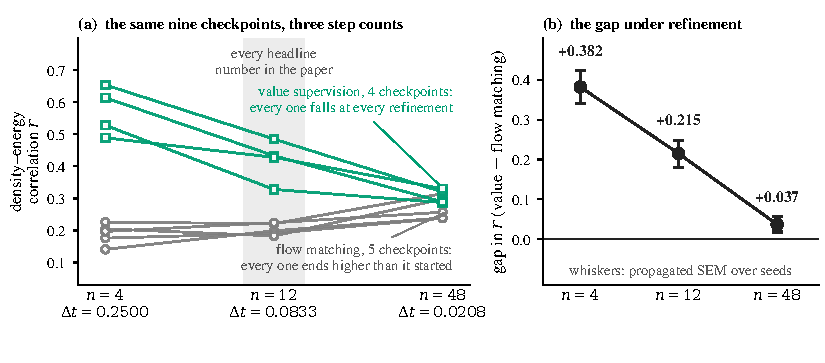
\includegraphics[width=\linewidth]{figures/out/figA_resolution.pdf}
\end{center}
\caption{\textbf{The paired resolution sweep.} The same nine checkpoints ---
five flow-matching controls (seeds $1$--$5$) and four value runs (seeds
$1$, $2$, $3$, $5$) --- re-scored at $n = 4$, $n = 12$ and $n = 48$ ODE steps on
identical parents, identical displacements and a pinned evaluation seed.
\textbf{(a)} Per checkpoint: all four value checkpoints fall at every
refinement, and all five flow-matching checkpoints end higher at $n = 48$ than
at $n = 4$, three of them monotonically. \textbf{(b)} The arm gap decays
$+0.382 \rightarrow +0.215 \rightarrow +0.037$. Each point is the difference of
the two arm means over independently trained seeds, five control and four
value, and each whisker is the propagated standard error over those seeds, a
descriptive SEM rather than a confidence interval. Every number reported
elsewhere in the paper is computed at $n = 12$. The value loss was itself
computed at $n = 4$, so one reading of the decay is that the ordering the term
teaches is expressed most strongly in the object the coarse estimator reports;
that is offered as a reading and not as a demonstrated mechanism. What the
analysis establishes is that the estimator is sensitive to solver resolution.
It does not distinguish model-dependent numerical error from an effect learned
under the four-step training estimator.}
\label{fig:resolution}
\end{figure}
